It has been over half a century since renowned astrophysicist Sjur
Refsdal first hypothesized the use of a supernova (SN) resolved into
multiple images as a cosmological tool. In recent years, the first
multiply-imaged core-collapse (CC) SN Refsdal \citep{Kelly:2015a}, and
subsequently the first Type Ia SN iPTF16geu \citep{Goobar:2016}, have
been discovered. As the light for each of the multiple
images follows a different path through the expanding universe and
through the lensing potential, the SN images appear delayed by hours
(for galaxy-scale lenses) or years (for cluster-scale lenses). These
gravitationally lenses are also important tools for observing
pair-instability (PI) and Population III (Pop III) SN in the early
universe (high-z), as \textbf{understanding these first stars is crucial to a
wide range of cosmology including the formation of primeval galaxies and the origin of
supermassive black holes} \cite{Whalen:2013}. As PI on an ongoing HST
Archival Research Grant, \textbf{I am developing the first open-source
software package} in Python (\textit{Supernova Time Delays} [SNTD])
that will be essential to making precise measurements of lens
properties and time delays for the hundreds of multiply-imaged SN
observations expected over the next decade (Figure 1). My research
will have two major components: 1. Using SNTD and multiply-imaged
SN as a cosmological probe. 2. Observing and understanding the
physical properties of very high-z PI and POP III SN.

\begin{wrapfigure}{r}{.5\textwidth}
\centering
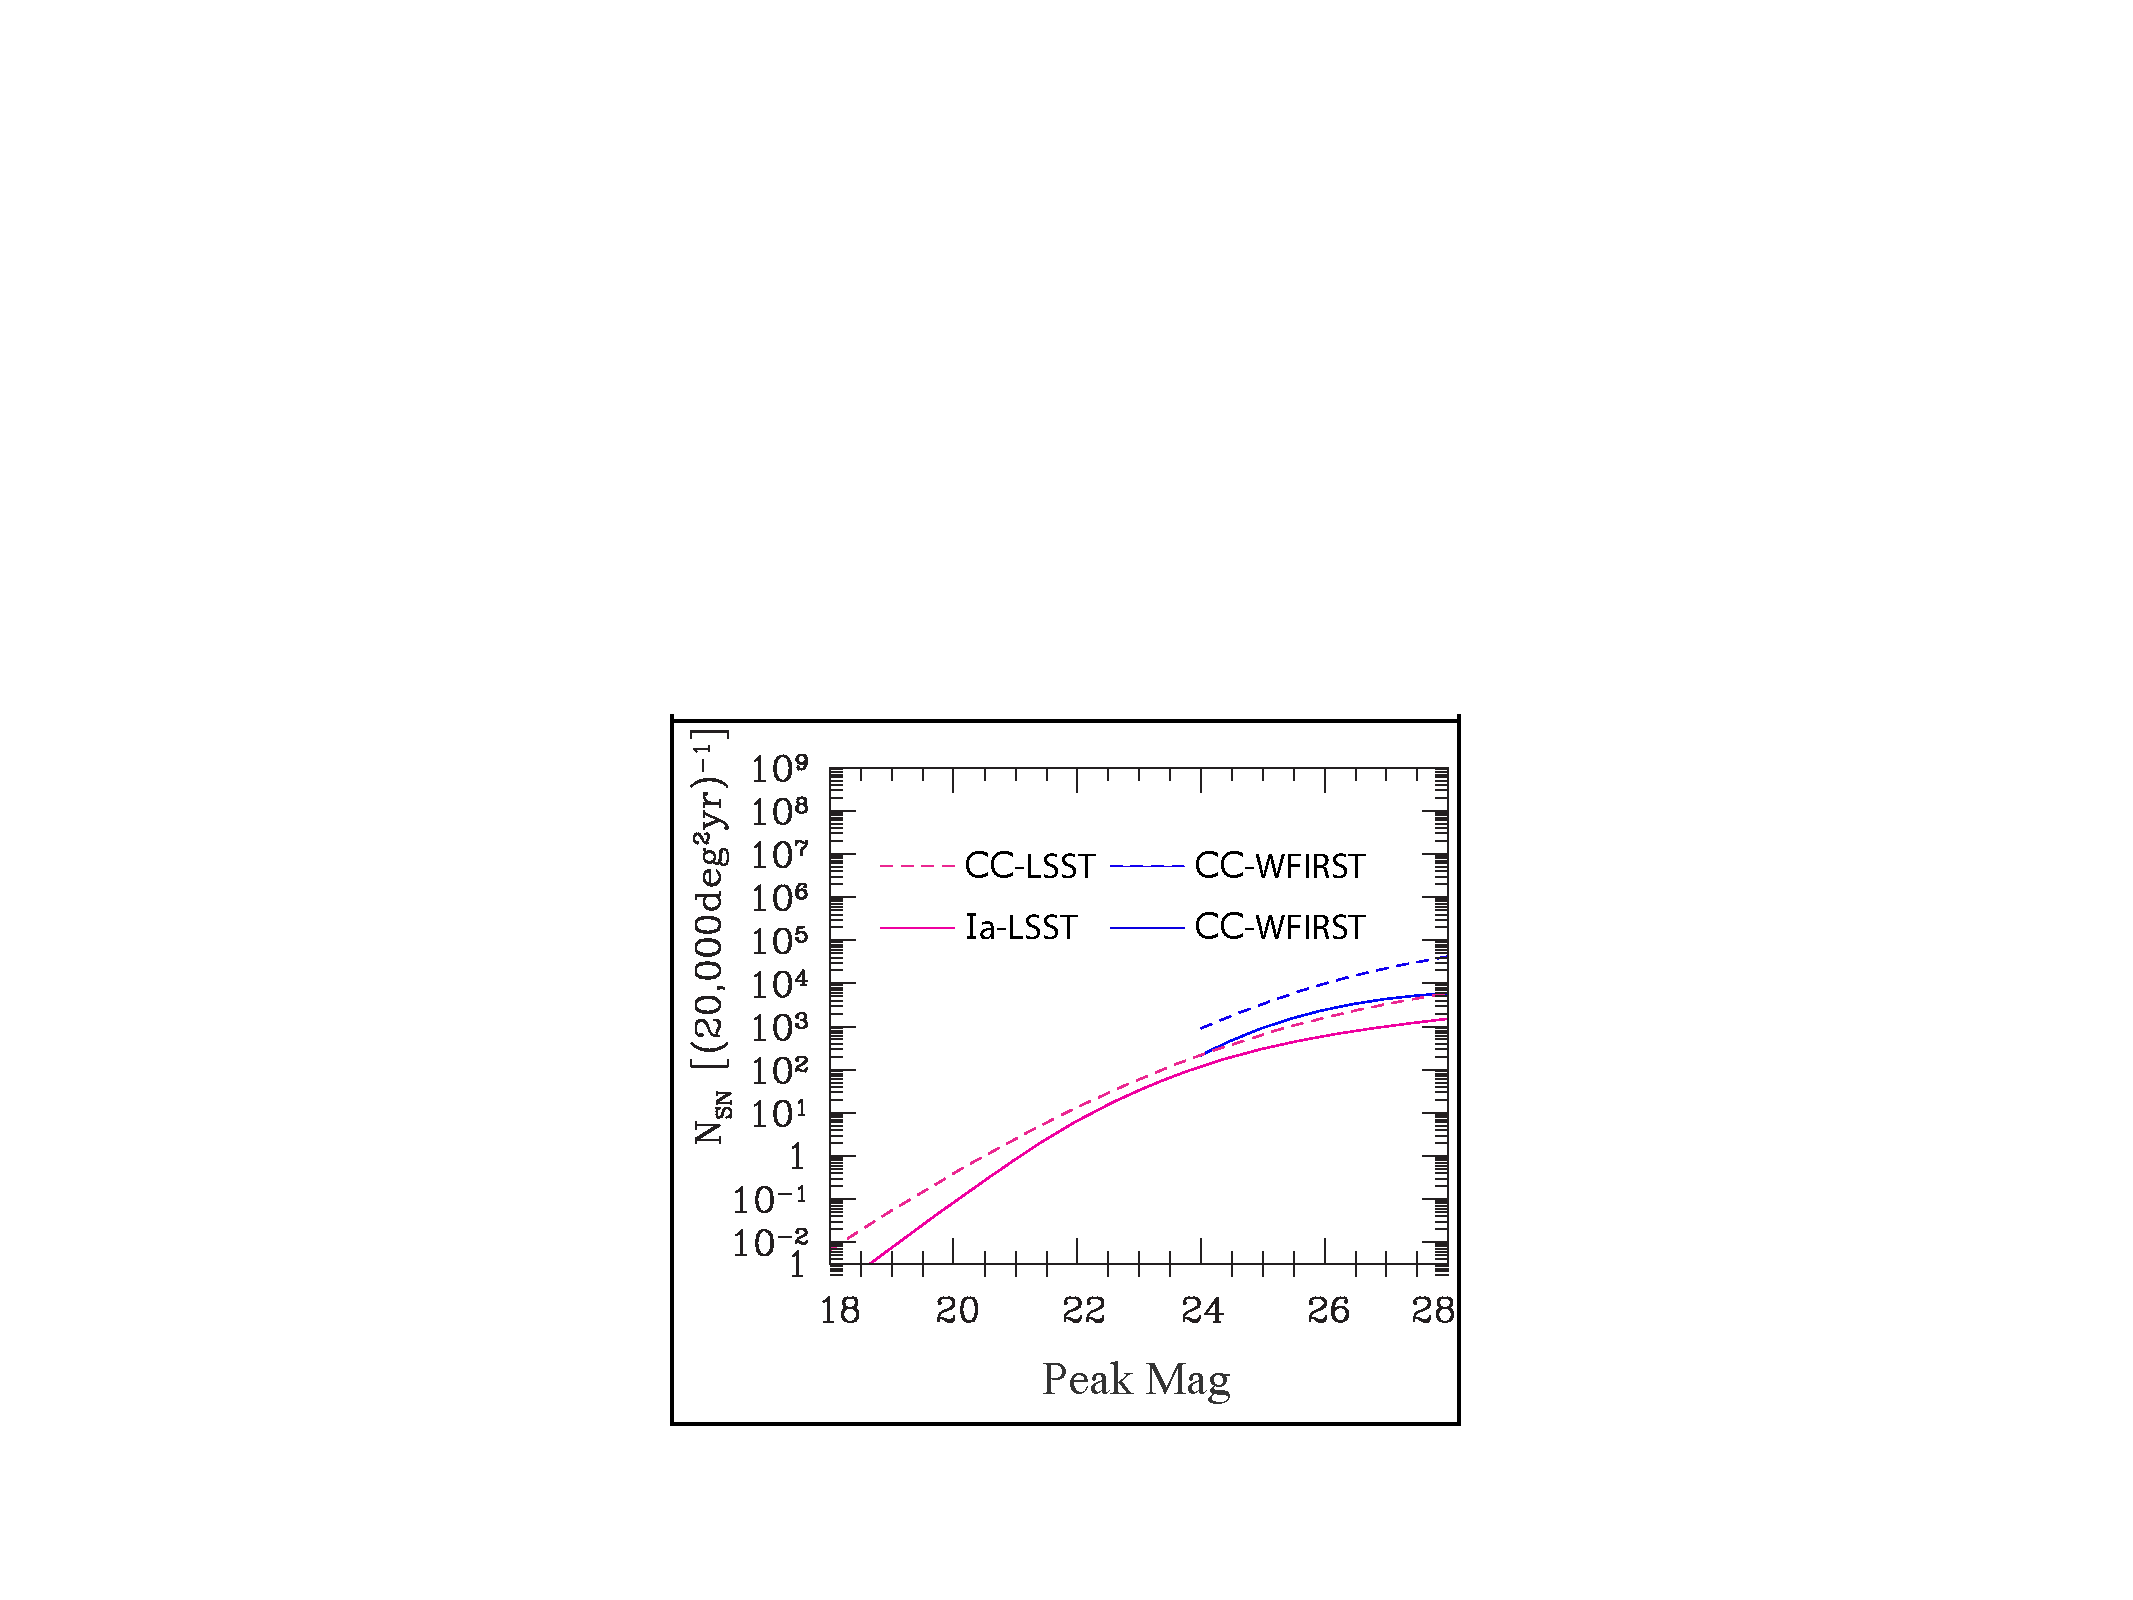
\includegraphics[height=.4\textwidth]{FIG/wfirst_lsst}
\caption{
\noindent\fontsize{10}{14}\selectfont
Expected numbers of lensed SN Ia and Core Collapse SN for LSST
$(i_{peak,lim})$ and WFIRST $(H_{peak,lim})$ after one year of
observations. With this huge volume of lensed CC and Ia SN
observations expected in the next decade, the open-source SNTD package
will be widely used and essential for analyzing this large WFIRST/LSST SN sample
(adapted from Oguri $\&$ Marshall 2010 \cite{Oguri:2010a}).}
\end{wrapfigure}

\noindent\underline{\textit{Intellectual Merit}} : After completing SNTD, I
will use the software to make more precise time delay measurements for
the two currently documented multiply-imaged SN. Properties of dark
energy and dark matter are still poorly understood and inadequately
constrained, but accurate measurements of the lensing magnification
and time delays for SN Refsdal can be used to test models for the dark
matter distribution in the lensing
object \cite{Rodney:2015a,Rodney:2016} or as a probe to test
cosmological models \cite{Suyu:2014}. As SN iPTF16geu is Type Ia,
achieving more accurate measurements will provide both an important
milestone in breaking degeneracies in the lens model and a result for
the Hubble constant $H_0$ that is completely independent of the local
distance ladder \cite{Kolatt:1998,Oguri:2003b}. The methodology and
software I develop will be \textbf{critical to future SN surveys} for
analyzing multiply-imaged SN and tightening the constraints found in
the course of this work.

Over the next 2 years, working with my
advisor Dr. Steven Rodney, I will be able to search for high-z and
strongly lensed SN in the 101-orbit HST program BUFFALO, which will
image the massive galaxy clusters of the Hubble Frontier Fields that
have delivered three of the most prominent examples of strongly lensed
transients: SN Refsdal \cite{Kelly:2015a}, the HFF14Spo
transients \cite{Rodney:2017}, and the lensed star
M1149-LS1 \cite{Kelly:2017}. Beginning in 2019, I will be
collaborating with the team of Dr. Rogier Windhorst on the JWST
Guaranteed Time Observations (GTO) program 1176.  This program will
apply 110 hours of cadenced imaging on massive galaxy clusters as well
as a deep field at the North Ecliptic Pole.  This could deliver
between 1 and 10 high-z detections of PISN\cite{Souza:2013}(Figure
2A). I will include theoretical light curve templates for both Pop III
and PI SN in SNTD, so that future observations can be identified and
both lens properties and progenitor physics studied.

\begin{wrapfigure}{r}{.5\textwidth}
\centering
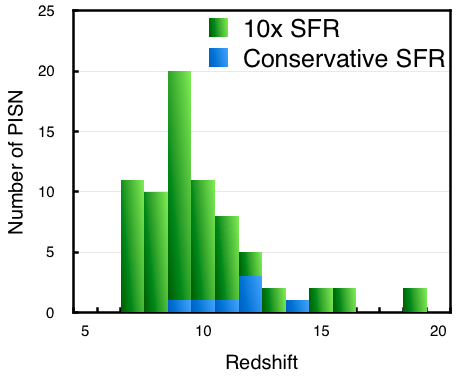
\includegraphics[height=.4\textwidth]{FIG/high_low_rates2}
%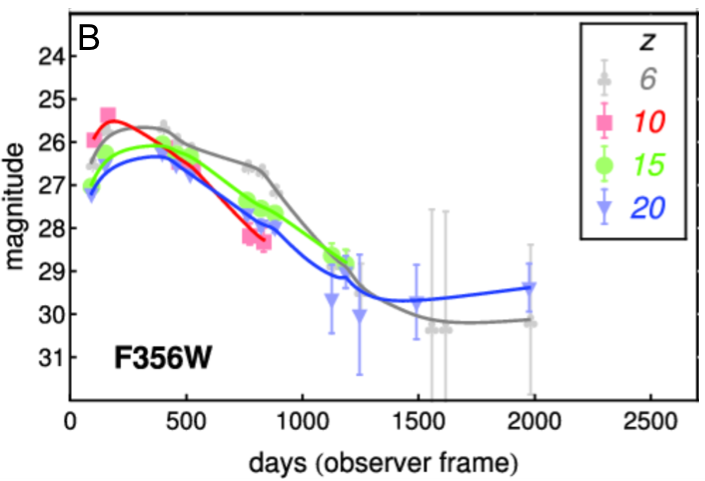
\includegraphics[height=.3\textwidth]{FIG/jwst_sim}
\caption{
\noindent\fontsize{10}{14}\selectfont
Histogram showing the dozens of expected PISN observations as a
function of redshift for a single JWST survey realization, covering
0.06$\%$ of the sky. Roughly 7 or 73 PISN observations with S/N$>$2
are expected per field when conservative and $10\times$ star formation
rates (SFR) are used respectively, over the course of 5
years. Therefore, we expect roughly 1-10 PISN observations during the
GTO survey (Figures adapted from Souza et
al. 2013 \cite{Souza:2013}).}
\end{wrapfigure}

\noindent\underline{\textit{Research Summary}}:
First, I will complete the python software package SNTD, and write a
publication presenting its capabilities and validation. Next I will
perform the reanalysis of SN Refsdal and SN iPTF16geu using SNTD,
writing a second publication presenting the more precise time delay
measurements, detailing the methodology required for these analyses,
and obtaining a constraint on $H_0$ from iPTF16geu. Finally, I will
add theoretical light curves for PI and POP III SN to the SNTD
package, and utilize the BUFFALO (HST) and GTO 1176 (JWST) programs to
study the physics of these first stars. From this last component of my
research, I will complete two further publications: one detailing the
catalog of PISN and POP III SN and their physical properties, and the
other making lens and time delay measurements for any strongly lensed
or multiply-imaged SN discovered. These \textbf{four publications}, as
well as the vetting and extensive use of the open-source SNTD package by the
entire community in future work with the next generation of space
telescopes, will be \textbf{clear measures of the success of this
work.}

\noindent\underline{\textit{Broader Impacts}}:
I will use my previous STEM outreach experiences (see personal
statement) to \textbf{increase the participation of young students in
astronomy and other STEM fields from a community comprised of 88$\%$
minorities underrepresented in STEM.}  My research is a terrific
gateway into STEM because it is naturally exciting and interesting:
space telescopes, pictures of galaxies, exploding stars, and
gravitational lensing are surefire topics to capture the attention and
imagination of a young learner, and I have already created a plan with
the local after-school program leader. First, I will take the kids to
our local University observatory and lead them through a series of
exciting and educational astronomical exercises. Once I have garnered
their attention and enthusiasm, I will have each student work on a
relatively simple astronomy project with me and at home, and then
present their results to community members. By creating a passion for
STEM and having participants choose and investigate a research
question, this outreach program will \textbf{improve the well-being of
the students by encouraging higher learning in STEM, and increase
public scientific literacy and public engagement with STEM} by
teaching the students and engaging the parents via the research
projects and presentations.

\noindent\fontsize{10}{14}\selectfont
[1]Kelly, P. L., et al. 2015, Science, 347, 1123 [2]Goobar, A., et
al. 2016, arXiv:1611.00014v1 [3]Oguri, M., $\&$ Marshall, P. J. 2010,
MNRAS, 405, 2579 [4]Rodney, S. A., et al. 2015, ApJ, 811,70
[5]Rodney, S. A., et al. 2016, ApJ, 820, 50 [6]Suyu, S. H., et
al. 2014, ApJ, 788, L35 [7]Kolatt, T. S., $\&$ Bartelmann, M. 1998,
MNRAS, 296, 763 [8]Oguri, M., $\&$ Kawano, Y. 2003, MNRAS, 338, L25
[9]Whalen, D. J., et al. 2013, arXiv:1312.6330 [10]de Souza, R. S., et al. 2013, MNRAS, 436, 1555
\pagebreak

%measure of success:


%Growing sample of gravitationally lensed publically available where tools would be available (rubin & haden-''The discovery of a gravitationaly lensed supernova Ia at redshift 2.22)

%First paragraph-->make it more of a thesis sentence at the end, instead of there is no current package. maybe also jwst high redshift sne for me to analyze.
